% contient la description des différentes possibilités pour traiter l'homographie unidirectionnelle au centre de la décomposition
%simon
%Homobox refait, une relecture s'impose, manque encore les ref vers les pseudos code (elles sont en com)
%Je sais pas si on doit garder la partie sur l'interp de hermite
\subsubsection{Séparation d'une homographie unidirectionelle}

On s'est ramené par la formule \ref{formule_decomposition_effective} à traiter des rotations et des homographies unidirectionnelles. Cette section présente une méthode de traitement pour les homograpghies unidirectionnelles.

\label{homobox_paragraph}

On considère une homographie unidirectionelle $h$, de la forme 
\begin{equation*}
h:(x,y)\mapsto \left(\frac{ax+p}{rx+t},\frac{dy+q}{rx+t}\right)
\end{equation*}

On peut décomposer cette homographie en deux applications $h_1 , h_2$
\begin{equation*}
h_1:(x,y) \mapsto \left(\frac{ax+p}{rx+t},y\right) \text{ et } h_2:(x,y) \mapsto \left(x,\frac{dy+q}{rx+t}\right)
\end{equation*}
On obtient $h=h_1  \circ h_2$, ce qui nous donne le schéma suivant 
\begin{equation*}
f\longrightarrow f'=f\circ h_1 \longrightarrow f''=f'\circ h_2
\end{equation*}
Chacune de ces deux transformations ne modifie l'image que dans une seule direction, cela permet d'effectuer des opérations sur des signaux unidimensionnels. Les méthodes de ré-échantillonnage sont donc plus simples, ce qui permet un gain de rapidité car les calculs sont moins coûteux. De plus, les transformations $h_1,h_2$ peuvent être appliquées en ne réalisant que des filtrages horizontaux et verticaux ; les direction de filtrage sont simples.
\begin{itemize}
\item Sur chaque colonne, la première transformation est une homographie en une dimension.
\item Sur chaque ligne, la seconde transformation est un zoom (d'un facteur différent selon la ligne).
\end{itemize}
On peut voir sur la figure \ref{image_separation_f14} l'effet des transformations $h,h_1,h_2$.

\begin{figure}[h!]
\centering
\subfigure[identité]{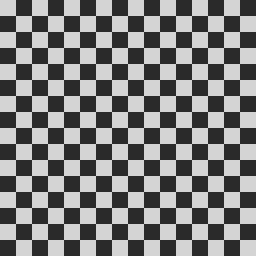
\includegraphics[scale=0.30]{damier.png}}
\subfigure[homographie unidirecionnelle $h=h_1 \circ h_2$]{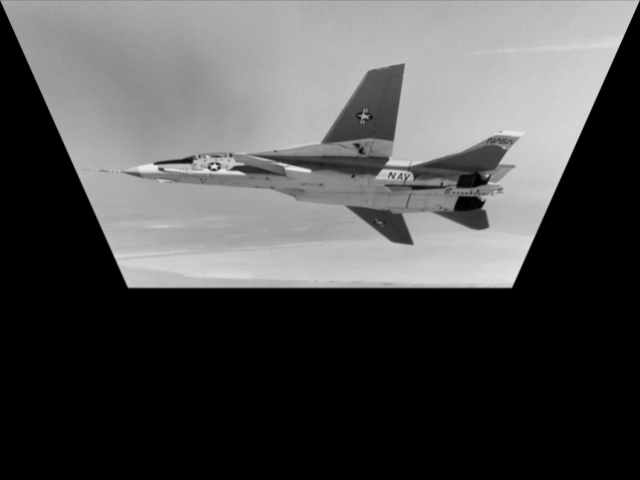
\includegraphics[scale=0.30]{homo_unidirec_f14_2.png}}
\subfigure[transformation $h_1$ ]{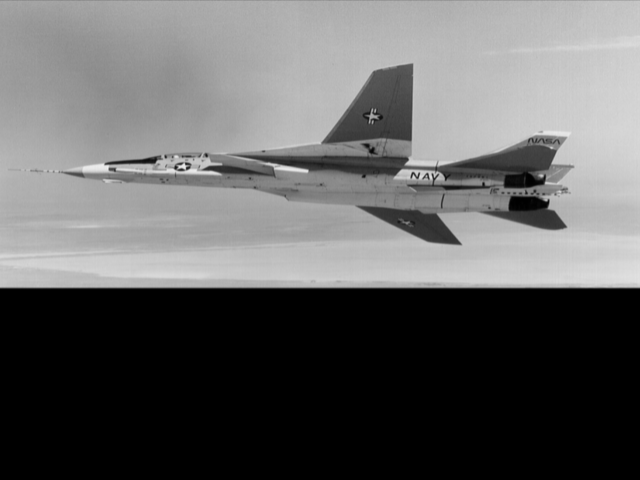
\includegraphics[scale=0.30]{homo_unidirec_part_1_f14_2.png}}
\subfigure[transformation $h_2$]{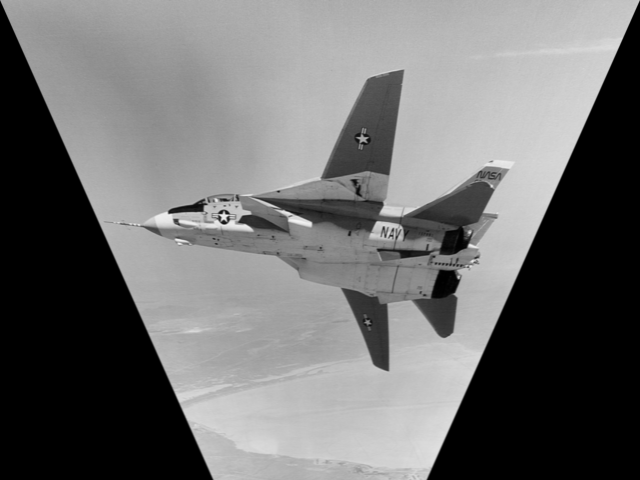
\includegraphics[scale=0.30]{homo_unidirec_part_2_f14_2.png}}
\caption{Séparation des homographies unidirectionnelles (échelle $0.3$) }
\label{image_separation_f14}
\end{figure}

\paragraph{Sous-échantillonnage gaussien}
\label{zoom_gaussien}
Le zoom gaussien est une méthode de sous-échantillonnage utilisant la convolution $f*G_{d}$ , où $G_d$ est un noyau gaussien d'écart type $d$. Dans nos algorithme on utilisera la méthode développée dans l'article \emph{SIFT is an invariant scale} \cite{morel2011sift}.

Si $f$ est une image on suppose que $f$ peut s'écrire sous la forme $f=G_{c'} * f'$, où $f'$ est une image de résolution infinie. Le paramètre $c'$ est le facteur de flou gaussien idéal de l'image $f$. L'expérience montre que le facteur de flou gaussien idéal se situe autour de $c=0.8$ \cite{morel2011sift}.\\
Soit $z\le 1$ posons $f''(x)=f'(zx)$. Si on cherche à échantillonner la fonction  $x\mapsto f(zx)$,  on doit d'abord s'assurer qu'elle possède un facteur de flou gaussien égal à $0.8$. On sait que 
\begin{equation*}
(f''*G_{c})(x)=(f'*G_{cz})(zx)
\end{equation*}
Grâce à cette relation, on peut en déduire la valeur de $d$ à utiliser, sachant que l'image de départ possède un flou gaussien de $c'$. On obtient
\begin{equation*}
(f*G_d)(zx)=(f'*G_c'*G_d)(zx)=(f'*G_{\sqrt{c'^2 + d^2}})(zx)
\end{equation*}
En identifiant ces deux expressions, on obtient
\begin{equation}
d=\sqrt{c^2 z^2 - c'^2}
\label{formule_zoom_gaussien}
\end{equation}

Le paramètre $c'$ est difficile à déterminer en pratique. L'expérience montre que pour une image "correctement échantillonnée", le facteur de zoom doit être pris égal à $0.7$. Cependant, pour certaines images provenant de la photographie, on peut prendre $c'=0.5$.

\paragraph{Ré-échantillonnage par les images intégrales}
\label{4Integral}
Dans ce paragraphe on présente une méthode permettant de ré-échantillonner une image 1D ; cette méthode s'appuie sur une approximation du zoom gaussien (cf. \ref{zoom_gaussien}) et utilise les images intégrales.

Soit $\Gcal_n^d$ le noyau définit par 
\begin{equation*}
\Gcal_1^d(x)=\frac{1}{d}\mathds{1}_{]-\frac{d}{2},\frac{d}{2}[}(x) \text{ et } \Gcal_{n+1}^d= \Gcal_n^d * \Gcal_1^d 
\label{formule_convol_n_int}
\end{equation*}
Cette suite de fonctions vérifie la propriété suivante
\begin{prop}
La fonction $x\mapsto \sqrt{n}~\Gcal_n^d(\sqrt{n}~x)$ converge uniformément sur $\mathbb{R}$ vers une courbe gaussienne 
\end{prop}
\begin{figure}
\centering
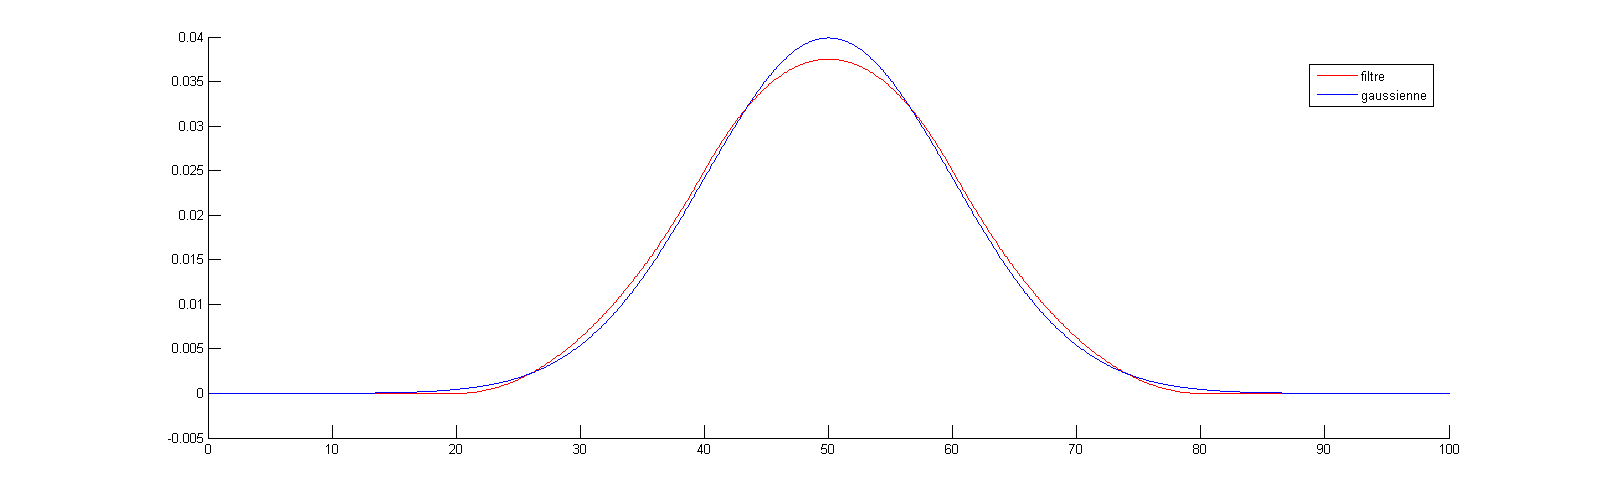
\includegraphics[width=10cm]{filtre_g3.png}
\caption{Comparaison en $\Gcal_3^20$ et $G_10$ (les filtres sont centrées sur $50$)}
\end{figure}
Si $f$ est une fonction continue par morceaux on définit $D_d$ l'opérateur de "dérivation discrète" par $D_d f(x)=\frac{f(x+\frac{d}{2})-f(x-\frac{d}{2})}{d}$  et on pose
\begin{equation*}
F_{n+1}(x)= \int_{-\infty}^{x}F_{n}(y)dy~~~~~~F_{0}(x)= f(x)
\end{equation*}
On a alors le lemme suivant 
\begin{prop} Pour toute fonction $f$ continue par morceaux à support compact :
\begin{equation}
 (f*\Gcal_n^d)(y)=D_d^n F_{n}(y)= \frac{1}{d^n}\underset{0 \le k\le n}{\sum} \binom{n}{k}(-1)^{k} F_{n}(y+\frac{(n-2k)d}{2})
\end{equation}
\end{prop}
\begin{proof}
Pour toute fonction $f$ continue par morceaux à support compact on a 
\begin{eqnarray*}
(f * \Gcal_1^d )(y)&=&\frac{1}{d} \int_{[y-\frac{d}{2},y+\frac{d}{2}]} f(x) dx\\
               &=&\frac{F_{1}(y+\frac{d}{2})-F_{1}(y-\frac{d}{2})}{d}\\
               &=&D_d F_{1}(y)
\end{eqnarray*}
On montre par récurrence que $ f*\Gcal_n^d=D_d^n F_{n}$.\\
La relation est donc vraie pour $n=1$, si la propriété est vraie au rang $n$ alors
\begin{equation*}
f*\Gcal_{n+1}^{d}=(f * \Gcal_{n}^d) * \Gcal_{1}^{d}= (D_d^n F_{n})*\Gcal_1^d 
\end{equation*}
Par linéarité de la convolution
\begin{equation*}
(f*\Gcal_{n+1}^{d}) = D_d^n (F_{n}*\Gcal_1^d) = D_d^{n+1} F_{n+1}
\end{equation*}
Comme $D_n^d$ est la somme des opérateurs de translation
\begin{equation*}
f\mapsto f(\cdot+\frac{d}{2})~~~~~~f\mapsto f(\cdot-\frac{d}{2})
\end{equation*}
On peut développer $D_d^n$ à l'aide du binome de Newton car les deux opérateurs commutent. On obtient donc
\begin{equation*}
(f*\Gcal_n^d)(y) = \frac{1}{d^n}\underset{0 \le k\le n}{\sum} \binom{n}{k}(-1)^{k} F_{n}(y+\frac{(n-2k)d}{2})
\end{equation*}

\end{proof}
Dans nos algorithmes, on utilisera généralement cette propriété pour $n=3$ mais on calculera l'opérateur $D_d^n$ en faisant des différences successives (algorithme \ref{pseudo_code_convol_4_int}).

On doit cependant calculer une valeur approchée des fonctions $F_{k}$  car on ne connait que les échantillons de la fonctions $f$.\\
Si le signal discret possède $m$ valeurs non nulles $f_k,k=0...m-1$, on peut poser 
\begin{equation*}
F_{0} (x) =\underset{0\le k \le m-1}{\sum}f_{k} \mathds{1}_{[k,k+1[}(x)
\end{equation*}

$(f_k)_{k=0...m-1}$ sont les termes du signal. On calcule ensuite $F_{n}(x)=\int_{-\infty}^{x}F_{n-1}(y)dx$, on a par exemple
\begin{equation*}
F_{1}(x)=\underset{k\le \lfloor x\rfloor \wedge m-1}{\sum}f_{k}+ f_{\lfloor x\rfloor}
(x-\lfloor x\rfloor)
\end{equation*}
Cette fonction est affine par morceaux. On peut démontrer la formule suivante par récurrence
\begin{eqnarray*}
F_{n}(x) &=& F_{n}(\lfloor x\rfloor \wedge m)~~+\mathds{1}_{[0,m[}(x) \underset{0\le k \le n-1}{\sum}F_{k}(\lfloor x \rfloor) \frac{(x-\lfloor x \rfloor)^{n-k}}{(n-k)!}\\
          &+&\mathds{1}_{[m,+\infty[}(x)\underset{1\le k \le n-1}{\sum}F_{k}(m) \frac{(x-m)^{n-1-k}}{(n-1-k)!}
\end{eqnarray*}
Où la valeur de $F_{n}$ se calcule par récurrence :
\begin{equation*}
\forall k \in \llbracket 0 ;m-1 \rrbracket, F_{n}(k+1)=F_{n}(k)+\underset{0\le l < n}{\sum} \frac{F_{l}(k)}{(n-l)!}
\end{equation*}
On doit calculer une composante constante par morceaux afin d'avoir la valeur de $F_{n}$ aux entiers ainsi qu'un terme polynomial de degré $n$ pour effectuer l'interpolation sur des valeurs non-entières.

Dans la pratique, on a utilisé cette formule pour $n=4$. Afin d'évaluer $F_4$, on procède de la façon suivante 
\begin{itemize}
\item Si $x\le 0$ alors $F_{n}=0$
\item Si $x\in ]0 , m[$ alors $F_{4}(x)-F_{4}(\lfloor x \rfloor)=P_{\lfloor x \rfloor}(x-\lfloor x \rfloor)$ où $P_k$ sont les polynômes de degré $4$ définis par
\begin{equation*}
P_k (r) =r \left( F_{3}(k) +\frac{r}{2} \left(F_{2}(k)+ \frac{r}{3}\left(F_{1}(k)+\frac{r}{4} f_{k}\right)\right)\right), k=0...m-1
\end{equation*}
\item Si $x\ge m$ alors $F_{4}(x)-F_{4}(m)=Q(x-m)$ où le polynôme $Q$ est défini par
\begin{equation*}
Q(r)=r \left(F_{3}(m)+\frac{r}{2} \left( F_{2}(m) + \frac{r}{3} F_1 (m)\right)\right)
\end{equation*}

\end{itemize}
Ces formules sont utilisées dans l'algorithme permettant d'évaluer l'intégrale quatrième de l'image (algorithme \ref{pseudo_code_eval_4_int}).

Pour calculer la valeur $F_4$ aux entiers, on peut applique la relation de récurrence suivante
\begin{eqnarray*}
F_{1}(k+1)&=&  F_{1}(k)+f_{k}  \\
F_{2}(k+1)&=&  F_{2}(k)+F_{1}(k)+\frac{f_{k}}{2}   \\
F_{3}(k+1)&=&  F_{3}(k)+F_{2}(k)+\frac{F_{1}(k)}{2}+\frac{f_{k}}{6}   \\
F_{4}(k+1)&=&  F_{4}(k)+F_{3}(k)+\frac{F_{2}(k)}{2}+\frac{F_{1}(k)}{6}+\frac{f_{k}}{24}  
\end{eqnarray*}
Ces formules sont utilisées dans le pseudo-code (algorithme \ref{pseudo_code_built_4_int}).

Dans cette méthode on ré-échantillonne le signal $(f_k)$ en l'interpolant d'abord par la fonction $F_{0}$, puis on ré-échantillonne en appliquant une convolution avec un noyau $\Gcal_n^d$. On utilise dans nos algorithmes les fonctions $\Gcal_3^d$ car elles se sont de bonnes approximations de courbes gaussiennes.\\ %placer figure 
Dans cette méthode, l'image est initialement interpolée par une fonction constante par morceaux. Lorsque le paramètre $d$ est choisi très petit, le ré-échantillonnage $F_{0}*\Gcal_3^d$ est équivalent à la méthode du point le plus proche.\\
On peut cependant corriger ce problème

\begin{prop}
Si on pose $\tilde{F}$ la spline d'ordre $1$ continue, telle que $\tilde{F}(k+\frac{1}{2})=f_k$ alors 
\begin{equation*}
( \tilde{F} * \Gcal_n^d ) (x) = D_d^{n}D_1 F_{n+1}(x)
\end{equation*}
Où $F$ est l'interpolation constante par morceaux de $(f)$ 
\end{prop}
\begin{proof}
On a
\begin{equation*}
\tilde{F}(x)=\displaystyle{\sum_{0\le k \le m-1}} f_k \Gcal_2^1 (x-k-\frac{1}{2})=(F_{0} *\Gcal_1^1 )(x)
\end{equation*}
On obtient alors 
\begin{equation*}
\tilde{F}*\Gcal_n^d=(F_{0}*\Gcal_1^1)*\Gcal_n^d=(F_{0}*\Gcal_n^d)*\Gcal_1^1=(D_d^n F_{n})*\Gcal_1^1= D_d^n D_1 F_{n+1}
\end{equation*}
\end{proof}
L'interpolation supplémentaire peut donc être obtenue en évaluant $F_{n+1}$. La méthode de calcul est donc la même que dans le cas précédent, la convolution avec $\Gcal_3^d$ nécessite l'utilisation l'intégrale quatrième de l'image dans la pratique.\\
Il est possible d'utiliser cette méthode pour obtenir une représentation plus régulière du signal de départ mais la courbe $F_0 * \Gcal_p^1~$ n'est pas interpolante si $2\le p$.\\
%à faire mieux 
Afin d'implémenter cette méthode, nous devons déterminer la valeur du paramètre $d$ en fonction du facteur de zoom local $z$ que l'on doit effectuer en ce point. $z$ sera choisi égal à la dérivé de la transformation au point où l'on ré-échantillonne.\\ 
On réutilise les résultats du paragraphe précédent (cf. \ref{zoom_gaussien}), car les  fonctions $\Gcal_3^d$ sont de bonnes approximations de courbes gaussiennes. L'écart type $\sigma$ de $\Gcal_3^d$ est donné par la formule 
\begin{equation*}
\sigma=\frac{d}{2}
\end{equation*}
Par la formule du zoom gaussien (formule \ref{formule_zoom_gaussien}), on en déduit que si $z\ge 1$, alors
\begin{equation*}
d=2\sqrt{c^2 z^2 - c'^2} \text{ avec } c=0.8 \text{ et } c'=0.7
\end{equation*}
La valeur de $c'$ peut être choisie en fonction de l'image d'entrée : pour des images très nettes, si l'on souhaite que le résultat final ne soit pas aliasé, on doit prendre une valeur de $c'$ autour de $0.5$. Pour la majorité des image utilisée lors de nos expériences une valeur de $0.7$ était suffisante. Une valeur trop faible de $c'$ aboutit à un flou excessif.
